\documentclass[a4paper,12pt]{article} % This defines the style of your paper

\usepackage[top = 2.5cm, bottom = 2.5cm, left = 2.5cm, right = 2.5cm]{geometry} 
\usepackage[utf8]{inputenc} %utf8 % lettere accentate da tastiera
\usepackage[english]{babel} % lingua del documento
\usepackage[T1]{fontenc} % codifica dei font

\usepackage{multirow} % Multirow is for tables with multiple rows within one 
%cell.
\usepackage{booktabs} % For even nicer tables.

\usepackage{graphicx} 

\usepackage{setspace}
\setlength{\parindent}{0in}

\usepackage{float}

\usepackage{fancyhdr}

\usepackage{caption}
\usepackage{amssymb}
\usepackage{amsmath}
\usepackage{mathtools}
\usepackage{color}

\usepackage[hidelinks]{hyperref}
\usepackage{csquotes}
\usepackage{subfigure}

\pagestyle{fancy}

%\setlength\parindent{24pt}

\fancyhf{}

\lhead{\footnotesize Machine Learning: Assignment 1}

\rhead{\footnotesize Giorgia Adorni}

\cfoot{\footnotesize \thepage} 

\usepackage{xcolor}
\usepackage{listings,lstautogobble}
\definecolor{gray}{gray}{0.5}
\colorlet{commentcolour}{green!50!black}
\colorlet{stringcolour}{red!60!black}
\colorlet{keywordcolour}{blue}
\colorlet{exceptioncolour}{yellow!50!red}
\colorlet{commandcolour}{magenta!90!black}
\colorlet{numpycolour}{blue!60!green}
\colorlet{literatecolour}{magenta!90!black}
\colorlet{promptcolour}{green!50!black}
\colorlet{specmethodcolour}{violet}

\newcommand*{\literatecolour}{\textcolor{literatecolour}}

\newcommand*{\pythonprompt}{\textcolor{promptcolour}{{>}{>}{>}}}

\lstdefinestyle{python}{
	language=python,
	showtabs=true,
	tab=,
	tabsize=4,
	basicstyle=\ttfamily\footnotesize,
	stringstyle=\color{stringcolour},
	showstringspaces=false,
	keywordstyle=\color{keywordcolour}\bfseries,
	emph={as,and,break,class,continue,def,yield,del,elif ,else,%
		except,exec,finally,for,from,global,if,in,%
		lambda,not,or,pass,print,raise,return,try,while,assert,with},
	emphstyle=\color{blue}\bfseries,
	emph={[2]True, False, None},
	emphstyle=[3]\color{commandcolour},
	morecomment=[s]{"""}{"""},
	commentstyle=\color{commentcolour}\slshape,
	emph={array, matmul, ones, T, transpose, float32},
	emphstyle=[4]\color{numpycolour},
	emph={[5]assert,yield},
	emphstyle=[5]\color{keywordcolour}\bfseries,
	emph={[6]range},
	emphstyle={[6]\color{keywordcolour}\bfseries},
	literate=*%
	{:}{{\literatecolour:}}{1}%
	{=}{{\literatecolour=}}{1}%
	{-}{{\literatecolour-}}{1}%
	{+}{{\literatecolour+}}{1}%
	{*}{{\literatecolour*}}{1}%
	{**}{{\literatecolour{**}}}2%
	{/}{{\literatecolour/}}{1}%
	{//}{{\literatecolour{//}}}2%
	{!}{{\literatecolour!}}{1}%
	{<}{{\literatecolour<}}{1}%
	{>}{{\literatecolour>}}{1}%
	{>>>}{\pythonprompt}{3},
	frame=trbl,
	rulecolor=\color{black!40},
	backgroundcolor=\color{gray!5},
	breakindent=.5\textwidth,
	frame=single,
	breaklines=true,
	basicstyle=\ttfamily\footnotesize,%
	keywordstyle=\color{keywordcolour},%
	emphstyle={[7]\color{keywordcolour}},%
	emphstyle=\color{exceptioncolour},%
	literate=*%
	{:}{{\literatecolour:}}{2}%
	{=}{{\literatecolour=}}{2}%
	{-}{{\literatecolour-}}{2}%
	{+}{{\literatecolour+}}{2}%
	{*}{{\literatecolour*}}2%
	{**}{{\literatecolour{**}}}3%
	{/}{{\literatecolour/}}{2}%
	{//}{{\literatecolour{//}}}{2}%
	{!}{{\literatecolour!}}{2}%
	{<}{{\literatecolour<}}{2}%
	{<=}{{\literatecolour{<=}}}3%
	{>}{{\literatecolour>}}{2}%
	{>=}{{\literatecolour{>=}}}3%
	{==}{{\literatecolour{==}}}3%
	{!=}{{\literatecolour{!=}}}3%
	{+=}{{\literatecolour{+=}}}3%
	{-=}{{\literatecolour{-=}}}3%
	{*=}{{\literatecolour{*=}}}3%
	{/=}{{\literatecolour{/=}}}3%
}

\lstnewenvironment{python}
{\lstset{style=python}}
{}

\newenvironment{sciabstract}{%
	\begin{quote} \bf}
	{\end{quote}}


\renewcommand\refname{References and Notes}

\newcounter{problem}
\newcounter{solution}

\newcommand\Problem{%
	\stepcounter{problem}%
	\textbf{\theproblem.}~%
	\setcounter{solution}{0}%
}

\newcommand\Solution{%
	\textbf{Solution:}\\%
}

\newcommand\ASolution{%
	\stepcounter{solution}%
	\textbf{Solution \solution:}\\%
}

\begin{document}
	\thispagestyle{empty}  
	\noindent{
		\begin{tabular}{p{15cm}} 
			{\large \bf Machine Learning} \\
			Università della Svizzera Italiana \\ Faculty of Informatics \\ 
			\today  \\
			\hline
			\\
		\end{tabular} 
		
		\vspace*{0.3cm} 
		
		\begin{center}
			{\Large \bf Assignment 1: Neural Networks}
			\vspace{2mm}
			
			{\bf Giorgia Adorni 
			(\href{mailto:giorgia.adorni@usi.ch}{giorgia.adorni@usi.ch})}
			
		\end{center}  
	}
	\vspace{0.4cm}
	
	%%%%%%%%%%%%%%%%%%%%%%%%%%%%%%%%%%%%%%%%%%%%%%%%
	%%%%%%%%%%%%%%%%%%%%%%%%%%%%%%%%%%%%%%%%%%%%%%%%
	
	\section{The Perceptron}
	Before working on a neural network we will study the perceptron; a linear 
	classifier
	without an activation function or a very simple single layer network as 
	given in Figure \ref{fig:perceptron}.
	You are given a dataset of size $n: \mathcal{D} = \{(\overline{x}_1 
	,\hat{y}_1),(\overline{x}_n ,\hat{y}_2),\dots , (\overline{x}_n 
	,\hat{y}_n)\}$, where input is represented as $k$-dimensional vectors 
	$\overline{x}_i \in \mathbb{R}^k$, and the targets $\hat{y}_i \in 
	\mathbb{R}$ are scalar. Assume bias term $b \in \mathbb{R}$ is not part of 
	weight matrix $\underline{W} = [w_1,w_2,\dots,w_k]^T$.
	
	\begin{figure}[H]
		\begin{minipage}[c]{.49\textwidth}
			\centering
			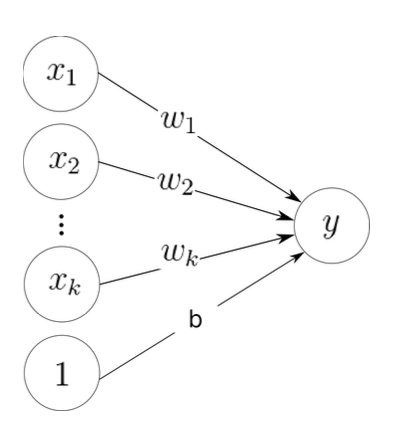
\includegraphics[width=.7\linewidth]{neuron.png}
			\captionof{figure}{The linear perceptron with single output}
			\label{fig:perceptron}
		\end{minipage}
		~
		\begin{minipage}[c]{.49\textwidth}
			\centering
			\begin{tabular}{|c|c|c|c|}
				\hline
				$\overline{x}_{i,1}$ & $\overline{x}_{i,2}$ & 
				$\overline{x}_{i,3}$ & $\hat{y}_i$ \\\hline
				-9         & -5         & 5          & 
				0                           \\\hline
				4          & -7         & -11        & 
				0                           \\\hline
				7          & 6          & -1         & 
				1                           \\\hline
				-9         & -5         & 4          & 
				1                           \\\hline
				-5         & -6         & -1         & 
				1                           \\\hline
				-4         & -4         & -8         & 
				0                           \\\hline
				5          & 7          & -9         & 
				1                           \\\hline
				2          & -4         & 3          & 
				0                           \\\hline
				-6         & 1          & 7          & 
				0                           \\\hline
				-10        & 6          & -7         & 
				1                           \\\hline
			\end{tabular}
			\captionof{table}{The training dataset}
			\label{tab:train-dataset}
		\end{minipage}
	\end{figure}
	\vspace{0.4cm}
	
	\Problem{What is the dimension of the output vector $\overline{y}$ if we 
	assume a batch of input data in form $\underline{x} \in \mathbb{R}^{d 
	\times k}$?}\medskip
	
	\Solution{The output shape of the vector $\overline{y}$ is $d$. Given as 
	input $d$ sample for each batch, since the output is just one, we have one 
	output for each 
	element in the batch, so $1 \times d$ output.}\vspace{0.4cm}
	
	\Problem{Write down the vectorised equation for the forward pass, if input 
	$\underline{x} \in \mathbb{R}^{d \times k}$ is batch of data, and 
	$\overline{1}_d$ is a length $d$ long vector of ones (watch out for 
	dimensions to match).}\medskip
	
	\Solution{
		\begin{equation}
		\overline{y}=\underline{x} \, \underline{W}+\overline{1}_d \, b \mbox{ 
		,}
		\end{equation}
		\\where:
		\begin{itemize}
			\item[-] $\overline{y}$ is the output vector; 
			\item[-] $\underline{x}$ is the input matrix;
			\item[-] $\underline{W}$ is the parameters matrix (weights);
			\item[-] ${b}$ is the bias;
			\item[-] $\overline{1}_d$ is a vector  with $d$ ones.
		\end{itemize}
		In this specific case, the equation does not have the multiplication by 
		the activation function $\sigma$, and the bias $b$ is a scalar and not 
		a transposed vector like in the general formula $\overline{y} = 
		\sigma(\underline{x} \, \underline{W} + \overline{1}_d \, 
		\overline{b}^T)$
	}\vspace{0.4cm}
	
	\Problem{Write down the vectorised equation for the MSE of the 
	perceptron.}\medskip
	
	\Solution{	
		\begin{equation}
		MSE = \frac{1}{2 \, d} \, 
		(\overline{y}-\hat{\overline{y}})^T(\overline{y}-\hat{\overline{y}})
		\end{equation}
	
		where:
		\begin{itemize}
			\item[-] $d$ is the number of samples in the batch; 
			\item[-] $\hat{\overline{y}}$ is the target vector; 
			\item[-] ${\overline{y}}$ is the predicted vector.
		\end{itemize}}\vspace{0.4cm}
	
	\Problem{Determine the derivative of the error function w.r.t weights 
	\textit{Hint: $\frac{\partial 
	\overline{x}^T\overline{x}}{\partial\overline{x}^T} = 
	2\overline{x}$}}\medskip
	
	\Solution{	
		\begin{itemize}
			\item weights:
			\begin{equation}
			\frac{\partial E}{\partial \underline{W}}= \frac{\partial 
				\overline{y}}{\partial \underline{W}}\frac{\partial E}{\partial 
				\overline{y}}
			\end{equation}
			\item bias:
			\begin{equation}
			\frac{\partial E}{\partial {b}}= \frac{\partial 
				\overline{y}}{\partial {b}}\frac{\partial E}{\partial 
				\overline{y}}
			\end{equation}
		\end{itemize}
		
		Since in both the cases, the second factor become 
		\begin{equation*}
		\frac{\partial E}{\partial \overline{y}} = \frac{\partial }{\partial 
			\overline{y}} 
		\frac{1}{2  \, d} (\overline{y} - \hat{\overline{y}})^T (\overline{y} - 
		\hat{\overline{y}})
		= 
		\frac{1}{2 \, d}\, 2 \, (\overline{y}-\hat{\overline{y}}) = \frac{1}{d} 
		\, (\overline{y}-\hat{\overline{y}})
		\end{equation*}
		and
		\begin{equation*}
			\frac{\partial \overline{y}}{\partial\underline{W}}= 
			\frac{\partial}{\partial\underline{W}}\underline{x} \, 
			\underline{W} + \overline{1}_d \, b = \underline{x}^T \mbox{ ,}
		\end{equation*}
		 
		\begin{equation*}
			\frac{\partial \overline{y}}{\partial{b}}=\overline{1}_d^T \mbox{ ,}
		\end{equation*}
	
		we obtain
		
		\begin{itemize}
			\item weights:
			\begin{equation}\label{equation: weights}
			\frac{\partial E}{\partial \underline{W}}= \frac{\partial 
			\overline{y}}{\partial \underline{W}}\frac{\partial E}{\partial 
			\overline{y}} = \frac{1}{d} \, \underline{x}^T \, (\overline{y} - 
			\hat{\overline{y}})
			\end{equation}
			
			\item bias:
			\begin{equation}\label{equation: bias}
			\frac{\partial E}{\partial {b}}= \frac{\partial 
			\overline{y}}{\partial {b}}\frac{\partial E}{\partial \overline{y}} 
			= \frac{1}{d} \, \overline{1}_d^T \, (\overline{y} - 
			\hat{\overline{y}})
			\end{equation}
			
		\end{itemize}
	}\vspace{0.4cm}
	
	\Problem{Write down the equation of the weight update by gradient 
	descent.}\medskip
	
	\Solution{	
		From the derivatives of the error function defined in the Equations 
		\ref{equation: weights} and \ref{equation: bias}, we can compute the 
		parameters update using the following formulas:
		\begin{itemize}
		\item weights:
			\begin{equation}
				\underline{W}^{\mathrm{NEW}}=\underline{W}^{\mathrm{OLD}}-\eta 
				\frac{\partial E}{\partial\underline{W}} = 
				\underline{W}^{\mathrm{OLD}} - \eta \, \frac{1}{d} \, 
				\underline{x}^T(\overline{y}-\hat{\overline{y}})
			\end{equation}
		\item bias:
			\begin{equation}
				{b}^{\mathrm{NEW}}={b}^{\mathrm{OLD}}-\eta 
				\frac{\partial E}{\partial {b}} = {b}^{\mathrm{OLD}}-\eta \, 
				\frac{1}{d} \, \overline{1}_d^T (\overline{y} - 
				\hat{\overline{y}})
			\end{equation}
		\end{itemize}
	}\vspace{0.4cm}
	
	\Problem{Suppose $k = 3\mbox{, }d =10$, with a batch of data given in Table 
	\ref{tab:train-dataset}. The initial weights are $w_1 = -0.1$, $w_2 = 
	-0.3$, $w_3 = 0.2$ and the bias weight is $b = 2$. Compute the weights 
	after one step of gradient descent with learning rate of $\eta = 0.02$ 
	(report their value up to 2 decimal points). \textit{Hint: 
	MATLAB/Octave/Python might come in handy here.}}\medskip
	
	\Solution{
		The updated weights are $[0.17, \; -0.03, \; 0.03]$ and the updated 
		bias is $1.97$.
		
		\begin{python}
import numpy as np
			
x = np.array([[ -9, -5,    5],
			   [   4, -7, -11],
			   [   7,   6,  -1],
			   [ -9, -5,    4],
			   [ -5, -6,  -1],
			   [ -4, -4,  -8],
			   [   5,   7,  -9],
			   [   2, -4,    3],
			   [ -6,   1,    7],
			   [-10,   6,  -7]], dtype=np.float32)
			   
y_hat = np.array([0, 0, 1, 1, 1, 0, 1, 0, 0, 1], dtype=np.float32)
	
W = np.array([-0.1, -0.3, 0.2], dtype=np.float32)
b = 2			
eta = 0.02
ones_d = np.ones(10)
y = np.matmul(x, W) + b
delta = y - y_hat

W_new = W - eta * np.matmul(x.T, delta) * (1 / d)
b_new = b - eta * np.matmul(ones_d.T, delta) * (1 / d)

print("New weights = ", W_new.round(2), " \nNew bias = %.2f" % b_new)
		\end{python}
		
	}\vspace{0.4cm}
	
	\Problem{Learning in multi-layer neural networks is usually done with help 
	of two methods: backpropagation and gradient descent. Describe briefly 
	what role in the learning process each of the two has (Should not be longer 
	than $6$ lines).}\medskip
	
	\Solution{Backpropagation is a procedure for computing the gradient of 
	complex functions in an efficient way. In particular it consists in 
	calculating the derivative of the error function with respect to the 
	parameters, applying repeatedly the chain rule.\medskip
	
	Gradient descent is an iterative optimization algorithm that tries to 
	improve the model performance finding a local minimum of a given loss 
	function, updating the network parameters (weights and bias) by using the 
	gradient of this function. }

\end{document}
